
\subsection{Design}

\subsubsection{Iteration 4}
Det indledende design af Calendar blev lavet i Iteration 4. I denne iteration blev events lavet uden tilknytning til en gruppe, og alle kunne derfor se alle events. I denne iteration var der heller ikke endnu implementeret widgets. Derfor blev kalenderen lavet med grundlæggende funktionalitet, og der blev taget udgangspunkt i user storien "Tilføj/Fjerne begivenheder".\newline
I figur \ref{fig:CalendarIterations} kan man se de scrum goals som kalenderen havde.

\begin{figure}[H]
    \centering
    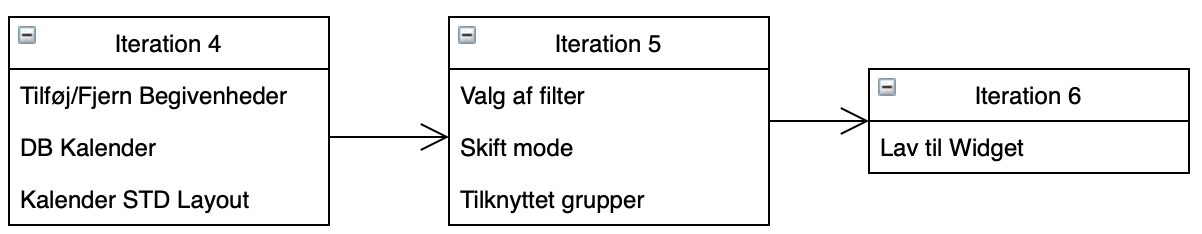
\includegraphics[width=1\linewidth]{10_Design_og_implementering/Calendar/Images/CalendarIterations.png}
    \caption{Calendar Iterations - Der ses at der i iteration 4 laves det grundlæggende funktionalitet for kalenderen, hvorefter 'ekstrafunktionalitet' opbygges}
    \label{fig:CalendarIterations}
\end{figure}{}

\mini{Evt. Flyt nogle af iterationsafsnit ned i bilag}

Derfor kan man altså se at de scrum goals, som var for Iteration 4 blev opfyldt, eftersom der blev lavet en kalender med layout, og der blev lavet en grundlæggende migration med events modellen. Der blev lavet en EventInsert action som gav alle brugere mulighed for at tilføje en event. I Iteration 4 var der altså en fungerende kalender, men en fælles for alle brugere. \newline

\subsubsection{Iteration 5}
I Iteration 5 havde man nu en fungerende kalender at tage udgangspunkt i fra iteration 4, og den kunne nu knyttes til grupper og gøres personlig.
Der blev tilføjet et gruppeId til events i en migration, og dette blev tilføjet til JSON modellen i javascriptet "GroupCalendar.js". For at finde events til den personlige kalender, kan man nu finde alle events for alle grupper en bruger er medlem af. Til gruppekalenderen, kan der blot findes alle events frem til den pågældende gruppe vha. gruppeId.
Til at lave typer, blev der tilføjet en "type" i modellen for events, som man derefter kunne filtrere events efter, derudover blev eventens farve (ThemeNo) sat efter hvilken type det er. 
I denne iteration blev der lavet en personlig kalender i navbaren, som man altid kunne tilgå, og der blev lavet en gruppekalender på gruppens side, men den manglede stadig at blive lavet til en widget.

\subsubsection{Iteration 6}
I den sidste iteration for kalenderens scrum goals, skulle kalenderen laves til en widget. Dette blev gjort ved at lave en ny entitet i databasen "Calendar", som alle andre widgets. Derudover skulle de 4 CRUD actions/views implementeres for kalenderen. Der blev lavet funktionalitet i widgetten, således at man på gruppens dashboard, kunne se på kalenderwidgetten om der er events i dag, og man på widgetten kunne tilgå gruppens personlige kalender.

\subsubsection{Iteration 7}
Der var ikke sprint goals for kalenderen i denne iteration, men der blev alligevel lavet små optimeringer, samt bug fixes som blev opdaget undervejs. Derudover blev hovedparten af databasekald flyttet hen i calendarrepository, for at overholde SRP.